\section{Sugeneruoti duomenys}
Buvo sugeneruotos dvi klases (grupes) po 15 duomenų įrašų (dvimačių taškų), kurie būtų tiesiškai atskiriami (n=2, m=30). Sugeneruoti taškai pavaizduoti grafiškai (žr. \ref{fig:pradinių taškų grafikas} pav.).

\subsection{Pradiniai taškai}
Žemiau pateikiami sugeneruoti duomenys (žr.~\ref{tab:klase0} ir~\ref{tab:klase1} lenteles). Lentelės duomenys buvo užpildyti naudojantis Claude\cite{claude_bendrai}.

\begin{table}[H]
    \centering
    \begin{minipage}{0.45\textwidth}
    \centering
    \captionof{table}{Klasės 0 duomenų taškai.}
    \begin{tabular}{|c|c|c|}
        \hline
        x1 & x2 & Klasė \\
        \hline
        -1.6026 & -2.1106 & 0 \\ \hline
        -1.4818 & -0.7816 & 0 \\ \hline
        -2.1873 & -2.1873 & 0 \\ \hline
        -0.7366 & -1.3861 & 0 \\ \hline
        -2.3756 & -1.5660 & 0 \\ \hline
        -2.3707 & -2.3726 & 0 \\ \hline
        -1.8064 & -3.5306 & 0 \\ \hline
        -3.3799 & -2.4498 & 0 \\ \hline
        -2.8103 & -1.7486 & 0 \\ \hline
        -2.7264 & -3.1298 & 0 \\ \hline
        -0.8275 & -2.1806 & 0 \\ \hline
        -1.9460 & -3.1398 & 0 \\ \hline
        -2.4355 & -1.9113 & 0 \\ \hline
        -2.9208 & -1.6994 & 0 \\ \hline
        -2.4805 & -2.2334 & 0 \\ \hline
    \end{tabular}
    \label{tab:klase0}
\end{minipage}
    \hfill
    \begin{minipage}{0.45\textwidth}
    \centering
    \captionof{table}{Klasės 1 duomenų taškai.}
    \begin{tabular}{|c|c|c|}
        \hline
        $x_1$ & $x_2$ & Klasė \\
        \hline
        $1,5186$ & $3,4818$ & 1 \\ \hline
        $1,9892$ & $1,1538$ & 1 \\ \hline
        $2,6580$ & $1,0233$ & 1 \\ \hline
        $2,1671$ & $0,4323$ & 1 \\ \hline
        $0,9375$ & $2,1575$ & 1 \\ \hline
        $2,5908$ & $2,1371$ & 1 \\ \hline
        $1,9075$ & $1,7591$ & 1 \\ \hline
        $0,8172$ & $1,4241$ & 1 \\ \hline
        $1,6315$ & $2,8457$ & 1 \\ \hline
        $2,2749$ & $0,5896$ & 1 \\ \hline
        $2,2593$ & $1,6919$ & 1 \\ \hline
        $1,4585$ & $2,4893$ & 1 \\ \hline
        $2,8248$ & $2,7450$ & 1 \\ \hline
        $1,3286$ & $1,7526$ & 1 \\ \hline
        $2,2650$ & $2,7804$ & 1 \\ \hline
    \end{tabular}
    \label{tab:klase1}
\end{minipage}
\end{table}

\subsection{Pradinių taškų grafikas}

Šiame grafike (žr.~\ref{fig:pradinių taškų grafikas} pav.) galima pamatyti iš viso 30 taškų:

\begin{itemize}
    \item Nulinė klasė – 15 taškų, mėlyna spalva.
    \item Pirmoji klasė – 15 taškų, raudona spalva.
\end{itemize}

\begin{figure}[H]
    \centering
    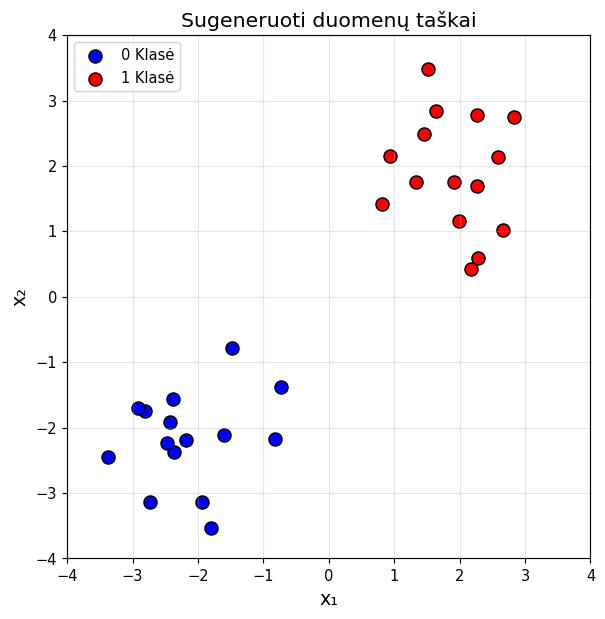
\includegraphics[width=0.5\textwidth]{../../grafikai/pradiniai_taskai.png}
    \caption{Sugeneruoti pradiniai duomenų taškai}
    \label{fig:pradinių taškų grafikas}
\end{figure}